\documentclass[mathserif]{beamer}
\usetheme{Luebeck}
%\documentclass{article}
%\usepackage{beamerarticle}
%\usepackage{graphicx}

\usepackage[francais]{babel}
\usepackage[utf8]{inputenc} % Uses the utf8 input encoding
\usepackage[T1]{fontenc} % Use 8-bit encoding that has 256 glyphs

\usepackage[nomath]{kpfonts}
\usepackage{eulervm}
\usepackage{amssymb}
%\usepackage{default}

\usepackage{amsthm}
\usepackage{amssymb}
\usepackage{xparse}
\usepackage{thmtools}
\usepackage{stackrel}

%shortcuts
\newcommand{\R}{\mathbb{R}}
\newcommand{\C}{\mathbb{C}}
\newcommand{\Z}{\mathbb{Z}}
\newcommand{\N}{\mathbb{N}}
\newcommand{\fii}{\varphi}
\newcommand{\dd}{\mathrm{d}}
\newcommand{\CP}{\mathbb{CP}}
\renewcommand{\S}{\mathbb{S}}
\DeclareMathOperator{\Sp}{Sp}
\DeclareMathOperator{\tr}{tr}
\DeclareMathOperator{\dist}{dist}

% theorems configuration

\makeatletter
\newtheoremstyle{indented}
{7pt} %vertical space before
{7pt} % vertical space after
{} %{\addtolength{\@totalleftmargin}{2.5em}
	%\addtolength{\linewidth}{-3.5em}
	%\parshape 1 3.5em \linewidth} %body font
{1.5em} %indent
{\bfseries} %header font
{.} %punctuation
{.5em} %horizontal space after header
{} %header specification

\theoremstyle{definition}

\newtheorem{defn}{Définition}[section]

\theoremstyle{plain}
%\newtheorem*{theorem*}{Theorem}

\newtheorem{thm}{Théorème}

\renewcommand{\thetheorem}{\Alph{theorem}}
\newenvironment{preuve}{
	\noindent \textbf{Preuve. }}{\hfill $\square$\medskip\par}

\newtheorem{exemple}[defn]{Exemple}
\newtheorem{prop}[defn]{Proposition}
\newtheorem{corr}[defn]{Corollaire}
\newtheorem{por}[defn]{Porisme}
\newtheorem{ex}[defn]{Exemple}
\newtheorem{lem}[defn]{Lemme}
\newtheorem{conj}{Conjecture}
\newtheorem{ax}{Axiome}  %Axioms have their own numerotation

\theoremstyle{definition}
\newtheorem{rem}[defn]{Remarque} %remarks are not indented
\newtheorem{rems}[defn]{Remarques}

%--------------
% Mise en page mathématique
%--------------
\addtolength{\jot}{.2em}


\title{Analyse microlocale et semiclassique}
\author[Alix Deleporte]{Alix Deleporte}
\institute[IRMA]{Institut de Recherche Mathématique Avancée\\Strasbourg}

\AtBeginSection
{
	\begin{frame}
		\frametitle{Plan}
		\tableofcontents[currentsection]
	\end{frame}
	
}

\newcommand{\spline}{\hline}
\renewcommand{\arraystretch}{1.3}
\begin{document}
\begin{frame}
	\titlepage
      \end{frame}

      \section{Mécanique classique et mécanique quantique}

      \subsection{Rappels de mécanique classique}

      \begin{frame}
        \frametitle{La mécanique classique}
        \begin{itemize}
        \item Mécanique : étude du déplacement d'objets.
          \uncover<2->{\item L'espace des configurations du système est
            de dimension paire. Exemple : position et vitesse en
            coordonnées.}
          \uncover<3->{\item Évolution temporelle : flot d'un champ
            de vecteurs}
          \uncover<4>{\item Cas conservatif : on préserve l'énergie.}
        \end{itemize}
      \end{frame}

      \begin{frame}
        \frametitle{Un exemple : le pendule simple}
        \begin{center}
          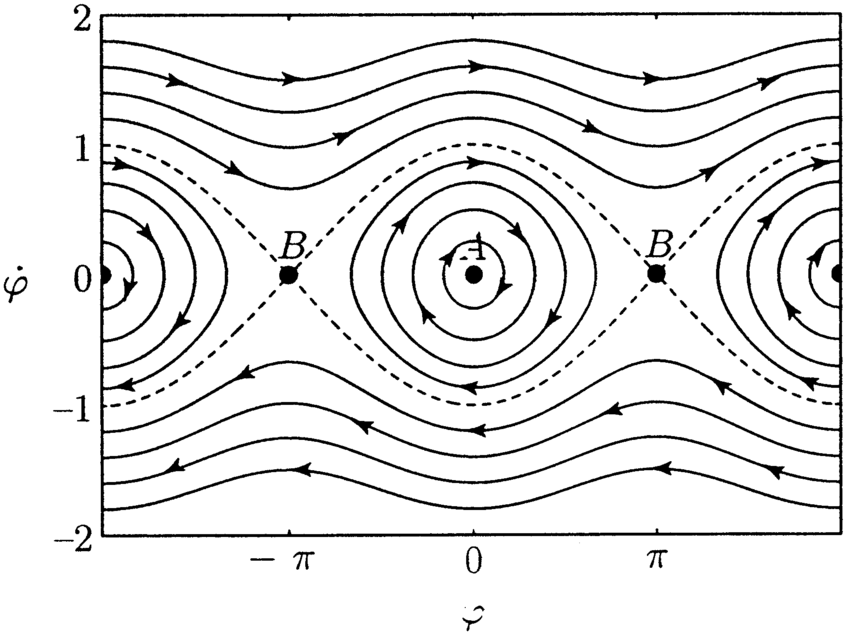
\includegraphics[width=0.7\textwidth]{pendulum.png}
        \end{center}
      \end{frame}

      \begin{frame}
        \frametitle{Géométrie symplectique}
        \begin{itemize}
        \item En dimension $>2*1$, les niveaux d'énergie ne
          suffisent plus à caractériser les trajectoires ; les
          équations du mouvement sont données par une information plus
          précise.
        \item Forme symplectique $\omega$ sur $M$: forme bilinéaire
          antisymétrique non-dégénérée sur les champs de vecteurs,
          fermée.
        \item Localement, on peut trouver une base
          $(X_1,\ldots,X_d,P_1,\ldots P_d)$ de champs de vecteurs avec
          $\omega(X_i,P_i)=1$ (toute autre combinaison fait zéro).
        \item Si l'énergie est $H$, le champ de vecteurs $X_H$ est
          défini par
          \[
            \omega(X_H,Y)=Y\cdot H.
          \]
        \end{itemize}
      \end{frame}

      \begin{frame}
        \frametitle{Particule massive dans un champ de potentiel}
        \begin{itemize}
        \item Espace des phases $\R^{n}_x\times \R^{n}_p$, forme symplectique
          \[
            \omega(\partial_{x_i},\partial_{p_i})=1.
          \]
          
        \item Énergie cinétique + énergie potentielle
          \[
            H=\frac 12 |p|^2 + V(x).
          \]
          
        \item Champ de vecteurs correspondant:
          \begin{align*}
            \dot{x}_i&=p_i\\
            \dot{p}_i&=-\partial_{x_i}V.
          \end{align*}
        \end{itemize}
      \end{frame}

      \subsection{Ondes et corpuscules}

      \begin{frame}
        \frametitle{Histoire de la lumière}
        \begin{description}
        \item[Grèce antique] Propagation en ligne droite, réflexion
          sur un miroir plan, absorbsion et diffusion.
        \uncover<2->{\item[Ibn al-Haytham (965-1040)] Lentilles et miroirs courbes.}
        \uncover<3->{\item[Newton] La lumière est faite de particules.
        \item[Huygens] La lumière est faite d'ondes qui se propagent.}
        \uncover<4->{\item[Newton, Young] Expériences de diffraction
          et d'interférences.}
      \uncover<5>{\item[Maxwell] Équations d'évolution de la lumière.}
        \end{description}
      \end{frame}

      \begin{frame}
        \frametitle{Principe de Huygens}
        \begin{center}
          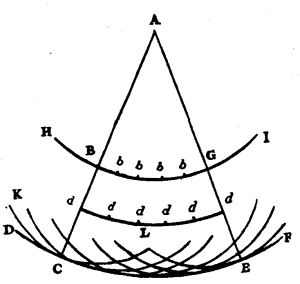
\includegraphics[width=0.6\textwidth]{Huygens.png}.
        \end{center}

      \end{frame}

      \subsection{Les principes de la mécanique quantique}
      \begin{frame}
        \frametitle{Interférences d'un électron}
        \begin{center}
          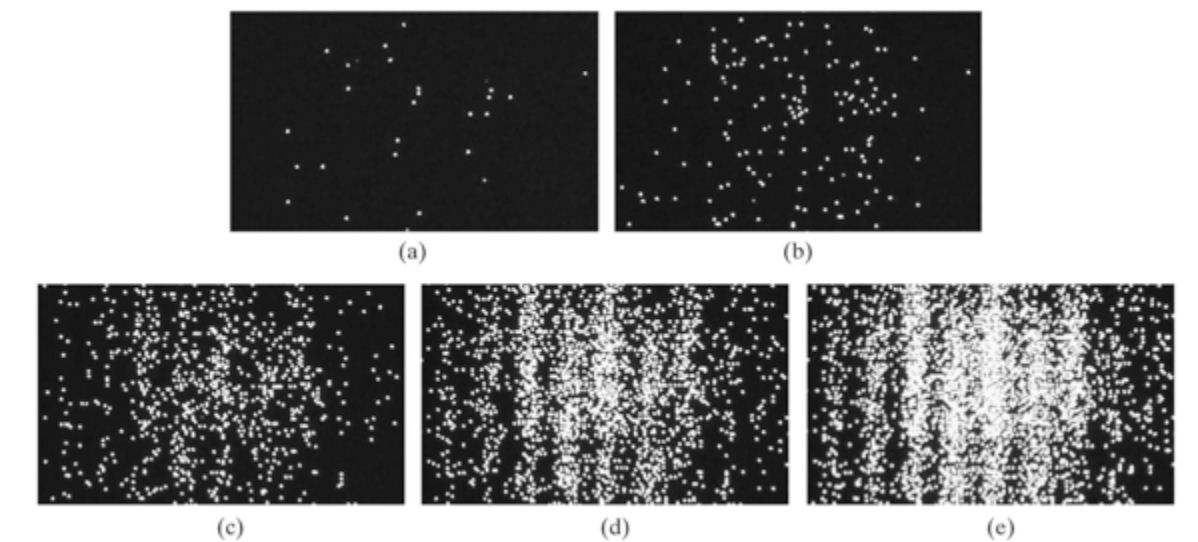
\includegraphics[width=0.8\textwidth]{electrons-slit.jpg}
        \end{center}
      \end{frame}
      \begin{frame}
        \frametitle{Description d'un système quantique}
        \begin{itemize}
        \item Espace des états : Hilbert $\mathcal{H}$.
        \item Énergie : Opérateur auto-adjoint $A$.
        \item Évolution : \[i\partial_t u = A u\]
          \item Exemple : $H=L^2(\R^n)$ et $A=-\hbar^2\Delta+V$.
        \end{itemize}
      \end{frame}

      \begin{frame}
        \frametitle{Principe de correspondance.}
        \begin{itemize}
        \item Les objets de la vie courante se déplacent \og en ligne
          droite\fg{}.
        \item Nécessité d'un équivalent quantique$\to$ classique du
          principe de Huygens.
        \end{itemize}
      \end{frame}

\section{Opérateurs à noyau et analyse microlocale}

\subsection{Transformée de Fourier}
\begin{frame}
  \frametitle{La transformée de Fourier}
  \begin{itemize}
  \item Idée de Fourier : représenter un signal (= une fonction du
    temps et/ou de l'espace) par ses fréquences.
  \item Composante de fréquence $\xi \in \R^d$ : onde monochromatique
    \[
      x\mapsto \exp(ix\cdot \xi).
    \]
    
  \item Transformation de Fourier:
    \[
      \widehat{f}(\xi)=\frac{1}{(2\pi)^{d/2}}\int_{\R^d}e^{-ix\cdot
        \xi}f(x) \dd x.
    \]
    
  \end{itemize}
\end{frame}

\subsection{Résolution intégrale d'équations différentielles}
\begin{frame}
  \frametitle{Équations différentielles intéressantes}
  \begin{itemize}
  \item Propagation des ondes:
    \[
      \cfrac{\partial^2 u}{\partial t^2}=\Delta u.
    \]
    
  \item Équation de la chaleur:
    \[
      \cfrac{\partial^2 u}{\partial t}=-\Delta u.
    \]
    
  \item Équation de Schrödinger libre:
    \[
      i\hbar\cfrac{\partial u}{\partial t}=\Delta u.
    \]
  \item Équation de Dirac libre:
    \[
      i\hbar\cfrac{\partial u}{\partial
        t}=(mc^2\alpha_0+c\alpha_1\partial_{x_1}+c\alpha_2\partial_{x_2}+c\alpha_3\partial_{x_3})u.
      \]
  \end{itemize}
\end{frame}

\begin{frame}
  \frametitle{Résolution par transformée de Fourier}
  Exemple pour l'équation de Schrödinger libre:
  Les ondes monochromatiques sont des fonctions propres des
    opérateurs de dérivation.
  \[i\partial_t
    \widehat{u}(\xi)=|\xi|^2\widehat{u}(\xi)\rightsquigarrow
    \widehat{u}(t,\xi)=e^{it|\xi|^2}\widehat{u}(0,\xi).\]
  \[u(t,x)=e^{-it|x|^2}\int e^{itx\cdot y}e^{it|y|^2}u(0,y)\dd y.\]

\end{frame}


\begin{frame}
  \frametitle{Autres résolutions par noyaux}
  Equation de Laplace : $\Delta u=0$ dans le disque, $u=f$ fixée sur le bord.

  Solution: noyau de Poisson:
  \[u(re^{i\theta})=\frac{1}{2\pi}\int_{\S^1}\cfrac{1-r^2}{1-2r\cos(\theta-t)+r^2}f(e^{it})\dd t.\]
\end{frame}


\subsection{Opérateurs pseudo-différentiels et OIF}

\begin{frame}
  \frametitle{Opérateurs pseudodifférentiels}
  L'opérateur différentiel $a(x)\partial_{x_j}$ s'écrit par une double
  transformée de Fourier:
  \[
    a(x)\partial_{x_j}f(x)=\int e^{i(x-y)\cdot \xi}(i\xi_ja(x))f(y)\dd
    y \dd \xi.
  \]

  Opérateurs pseudodifférentiels : on généralise à une fonction
  quelconque de $x,\xi,y$ :

  \only<2-3>{\[
    Pf(x)=\int e^{i(x-y)\cdot \xi}p(x,\xi,y)f(y)\dd y \dd \xi.
  \]}

\only<4>{\[
    P_{\hbar}f(x)=\int e^{\frac{i}{\hbar}(x-y)\cdot
      \xi}p_{\hbar}(x,\xi,y)f(y)\dd y \dd \xi.
    \]}

  \uncover<3-4>{On peut calculer la composée de deux pseudodiff dans
    la limite \only<3>{des
    grandes fréquences} \only<4>{$\hbar\to 0$}.}

\end{frame}

\begin{frame}
  \frametitle{Phase stationnaire}
  Méthode de la phase stationnaire : étude des intégrales du type
  \[
    \int e^{it\phi(x)}a(x)\dd x
  \]
  dans la limite $t\to +\infty$.

  Là où $d\phi \neq 0$ on peut faire des intégrations par parties successives et
  sortir autant de facteurs $t^{-1}$ que l'on veut.

  Les points où $d\phi=0$ donnent une contribution qui a un
  développement asymptotiques en puissances de $t^{-1}$.

  C'est l'ingrédient essentiel dans l'étude des opérateurs
  pseudo-différentiels et leurs généralisations.
\end{frame}

\begin{frame}
  \frametitle{Réflexion sur un miroir}
  \begin{itemize}
  \item 
  Source en $S$ qui émet une onde de pulsation $\omega$, oeil en
  $E$.
\item 
  Chaque chemin $\gamma $ de $S$ à $E$ donne une contribution
  $\frac{e^{i\omega\ell(\gamma)}}{\ell(\gamma)^2}.$
\item 
  Quand $\omega\to +\infty$, les seuls chemins qui comptent sont de
  longueur critique.
  \end{itemize}
\end{frame}

\section{Application : formules de l'indice}
\begin{frame}
  \frametitle{Indice d'opérateurs}
  \begin{itemize}
  \item Un opérateur linéaire continu $A$ est dit \emph{de Fredholm} lorsque son
    noyau $\ker A$ et l'orthogonal de l'image $\text{coker A}$ sont de
    dimension finies.
  \item Exemple : l'application dérivée de $C^1_{per}([0,1])\mapsto
    C^0_{per}([0,1])$ a un noyau de dimension $1$ et un conoyau de dimension
    $1$.
  \item On appelle \emph{indice} d'un op\'erateur de Fredholm la
    diff\'erence $\dim \ker A-\dim \text{coker} A$.
  \item Exemple : $d_{DR}:H^{pair}(M)\mapsto H^{impair}(M)$ a comme indice
    de Fredholm $\chi(M)$.

  \end{itemize}
\end{frame}

\begin{frame}
  \frametitle{Indices de diff\'erentielles et laplacien}
  \begin{itemize}
  \item Si $A:E\mapsto F$ est de Fredholm avec $E$ et $F$ des Hilbert
    alors $A^*A$ et $AA^*$, autoadjoints, ont le m\^eme spectre
    except\'e un surplus de valeurs propres nulles ; donc par exemple,
    pour tout $t\in \R$, on a
    \[
      ind(A)=\tr e^{-tA^*A}-\tr e^{-tAA^*}.
    \]
    
  \item Si $A$ est une diff\'erentielle alors $A^*A$ et $AA^*$ sont
    des laplaciens.
  \item Pour conna\^itre la classe d'Euler il suffit de ma\^itriser le
    comportement en temps long de l'\'equation de la chaleur.
  \end{itemize}
\end{frame}

\begin{frame}
  \frametitle{Formule de Chern-Gauss-Bonnet}
  \begin{itemize}
  \item Pour obtenir $\chi(M)$ il faut regarder la diff\'erentielle
    sur un fibr\'e de type spineur.
  \item Si $M$ est de dimension $2k$, alors\[
      \chi(M)=(2\pi)^{-k}\int_M Pf(\Omega).
    \]
    
  \item $Pf$ d\'enote le \emph{Pfaffien} d'une matrice antisym\'etrique $(X_{i,j})$,
    avec
    \[
      \left(\sum X_{i,j}e_i\wedge e_j\right)^{\wedge k}=k!Pf(X)
      e_1\wedge \cdots \wedge e_{2k}.\]
  \item $\Omega$ est un tenseur de courbure.
  \end{itemize}
\end{frame}
\end{document}